\documentclass[12pt]{article}
\usepackage{amssymb}
\usepackage{amsmath}
\usepackage{graphicx}
\usepackage{subfigure}
\usepackage{float}
\usepackage[margin=1in]{geometry}
\author{Tianyu Dai, Xiaoqing Li, Yuheng Liao, Xuejian Ma}
\title{PHY566 - Percolation}
\begin{document}
\date{4/12/2017}
\maketitle
Percolation theory describes the behavior of connected cluster in a random graph. It usually concerns the movement and filtering of fluids through porous materials. In this project, we simulate the percolation transition and try to analyze its properties.
\section{Determine the critical probability $p_c$}
The basic idea to simulate the percolation transition is to take a $N\times N$ lattice, and then occupy the lattice sites at random according to a certain probability $p$. If a cluster of occupied sites spans the entire lattice from edge to edge, it's called a spanning cluster. The probability of the appearance of a spanning cluster rises with the rise of $p$. When $p$ is relatively small, it is highly unlikely to get a spanning cluster. However, for $p$ large enough, the existence of spanning cluster is guaranteed. The transition from one regime to the other is rather sharp and occurs at a critical concentration, which we call $p_c$. For $N\times N$ lattice, our basic task is to simulate the percolation transitions with different probability $p$, and figure out the $p_c$. Doing those for different $N$, and then plot $p_c - N^{-1}$ graph. From $p_c(N^{-1})$ graph, we can extrapolate to the infinite size limit $p_c(0)$.\\
\subsection{Basic Algorithm}
\indent The program details we should follow for $N\times N$ lattice is as below:\\
\begin{enumerate}
\item Begin with an empty $N\times N$ lattice and initialize all sites to zero, i.e. unoccupied.
\item Select and occupy a random site, labeling it with a cluster number.
\item Select another site at random and check neighboring sites to see if any belongs to a cluster created before. If not, the new site should be labeled with another cluster number. If so, we need to discuss among the following two situations:

\begin{enumerate}
\item If there's only one cluster number among all neighboring sites, give this number to the new site.
\item If there are several cluster number among all occupied neighbors, the new site is considered as a site bridge which connects multiple clusters into one. We should choose a common unique cluster number for resulting cluster, and then also give this number to the new site and relabel all sites in merged cluster to that number.
\end{enumerate}

\item Repeat step 3 until a common cluster number{} appears on all edges of the lattice.
\item The common cluster number is the number of the spanning cluster, and the fraction of all occupied sites among all lattice sites is $p_c$
\end{enumerate}

\subsection{Revised Algorithm}
To simplify the model and save computation time, we revised the original algorithm. \\
The original $N\times N$ lattice is expanded to $(N+1)\times(N+1)$ first. Each site on the boundary is labeled a unique number, as shown in Fig. (\ref{Boundary1})
\begin{figure}[H]
\centering
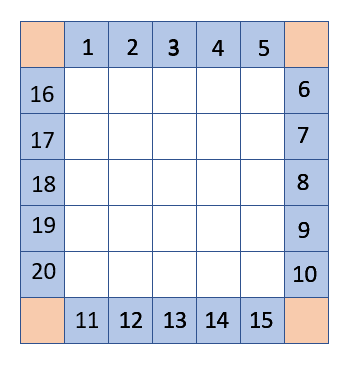
\includegraphics[width=0.5\textwidth]{Boundary1}
\label{Boundary1}
\caption{Boundary Setting}
\end{figure}

Then, follow below steps: 
\begin{enumerate}
  \item Select and occupy a random site from the lattice and label it as $4N+1+n$, which can distinguish it from the boundary. n is the step number. 
  \item Store the cluster number of four nearest sites. 
  \item Transverse all the occupied sites(including boundary sites). Relabel all sites which has the same cluster number as nearest sites to be the newest cluster number $4N+1+n$. \\
        The lattice before transverse and after transverse is shown in Fig. (\ref{Boundary2}). 
  \item If the maximum label on each boundary is the same as the newest cluster number, the spanning cluster shows up. The appearance of spanning cluster in the lattice and the spanning cluster is Fig. (\ref{Spanning}). 
  \item Repeat steps from the beginning. 
\end{enumerate}
\begin{figure}[h]
\centering
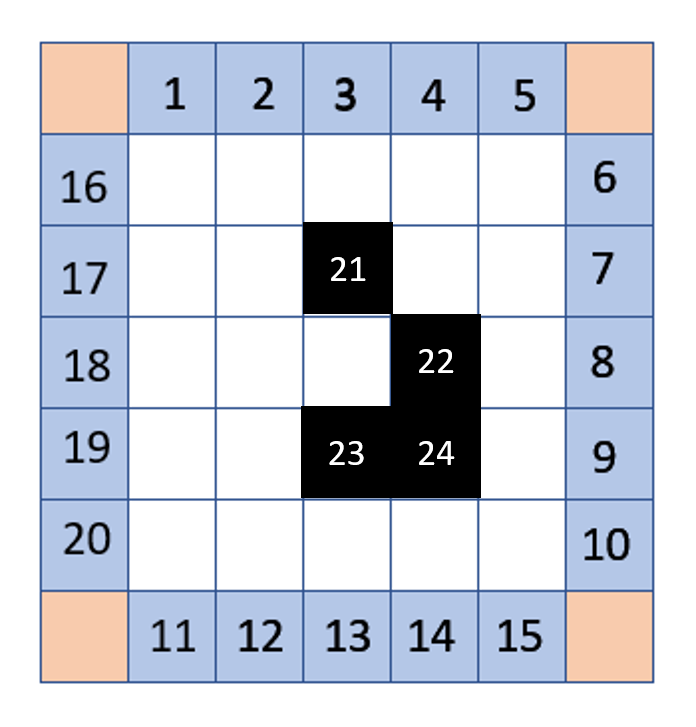
\includegraphics[width=0.4\textwidth]{Boundary2}
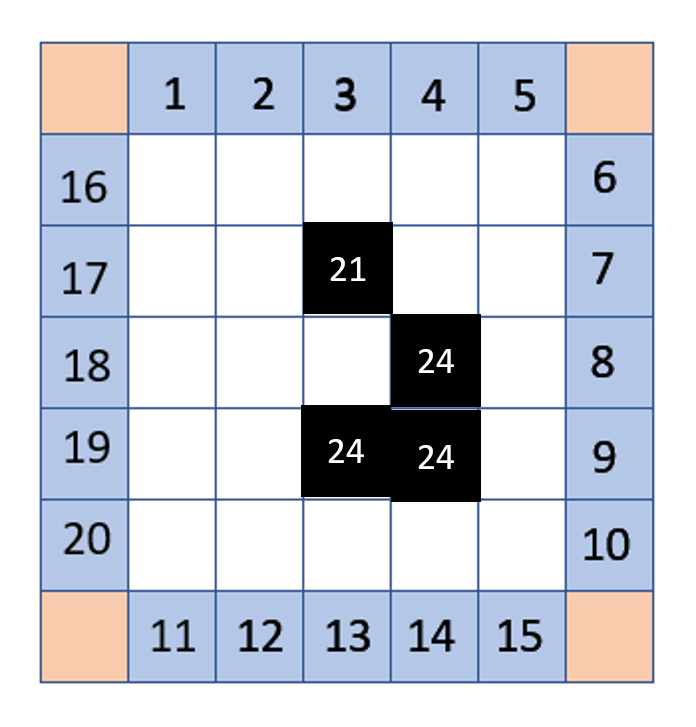
\includegraphics[width=0.4\textwidth]{Boundary3}
\caption{Cluster labels before and after the transverse}
\label{Boundary2}
\end{figure}

\begin{figure}[h]
\centering
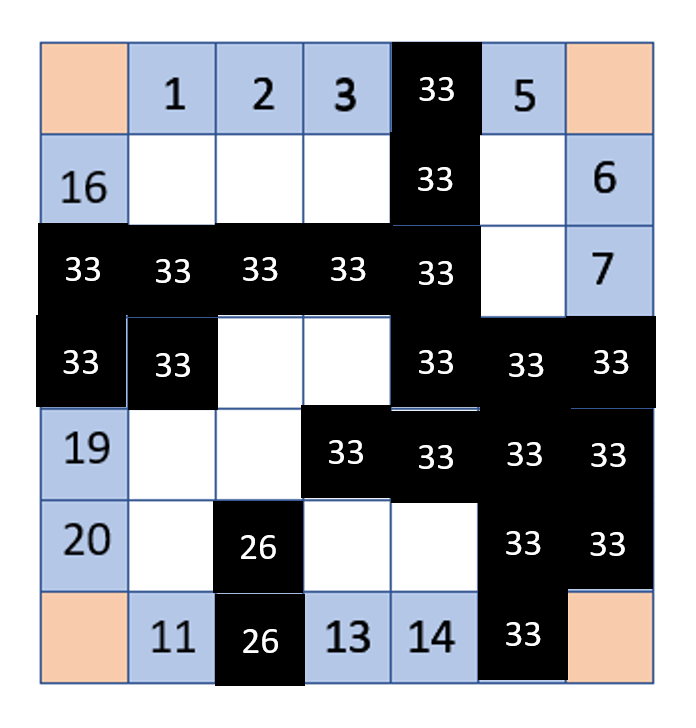
\includegraphics[width=0.4\textwidth]{Spanning1}
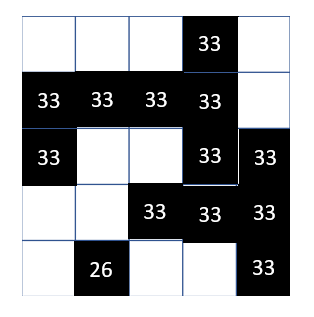
\includegraphics[width=0.4\textwidth]{Spanning2}
\caption{The spanning cluster}
\label{Spanning}
\end{figure}

The revised algorithm avoid dealing with boundary conditions. When the newest added site reaches the boundary, the lattice before and after transverse is shown in Fig. (\ref{Boundary3}). \\
\begin{figure}[h]
\centering
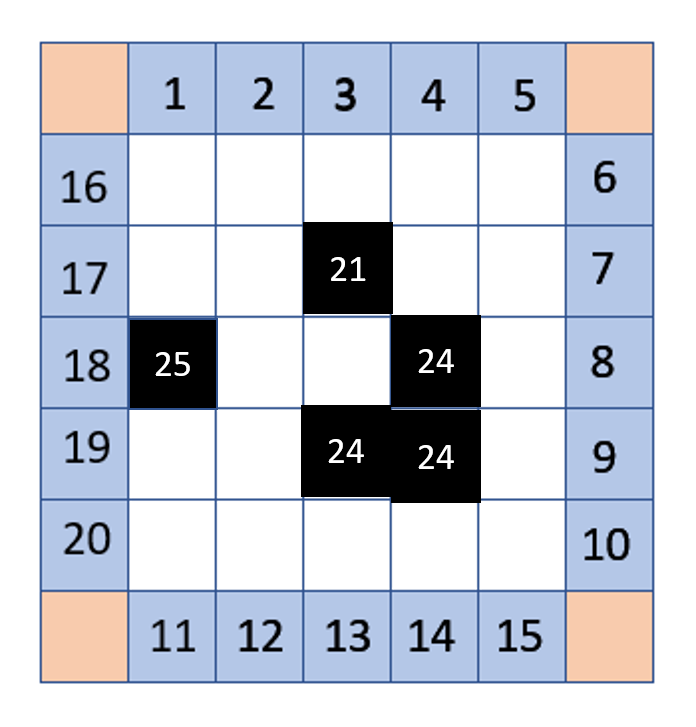
\includegraphics[width=0.4\textwidth]{Boundary4}
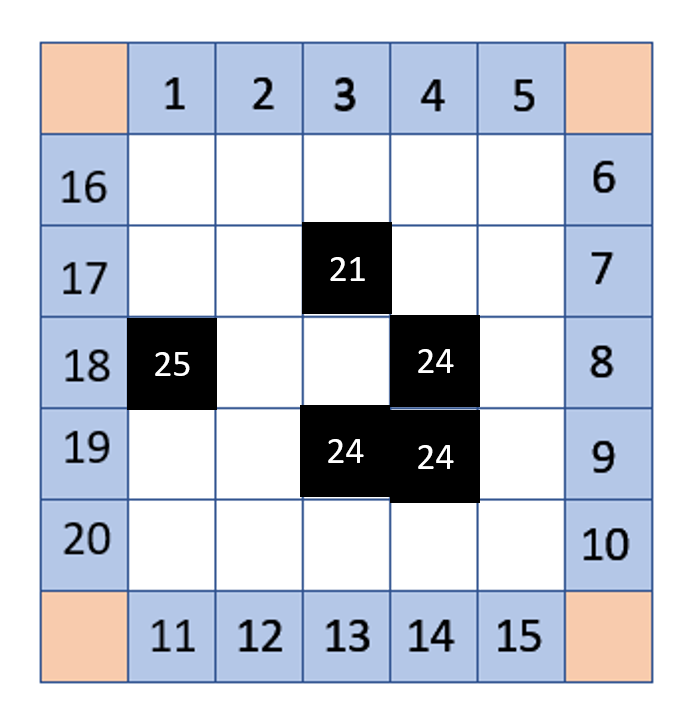
\includegraphics[width=0.4\textwidth]{Boundary5}
\caption{Newest added site reaches the boundary, before and after the transverse}
\label{Boundary3}
\end{figure}
The judge of how many nearest sites are occupied is also avoided. After each transverse, all cluster connected to the newest added site will be updated in each step. \\
Following the steps above, we can get the spanning clusters for different $N\in\{5, 10, 15, 20, 30, 50, 80\}$ as below:
\begin{figure}[H]%[!htb]
\minipage{0.5\textwidth}
  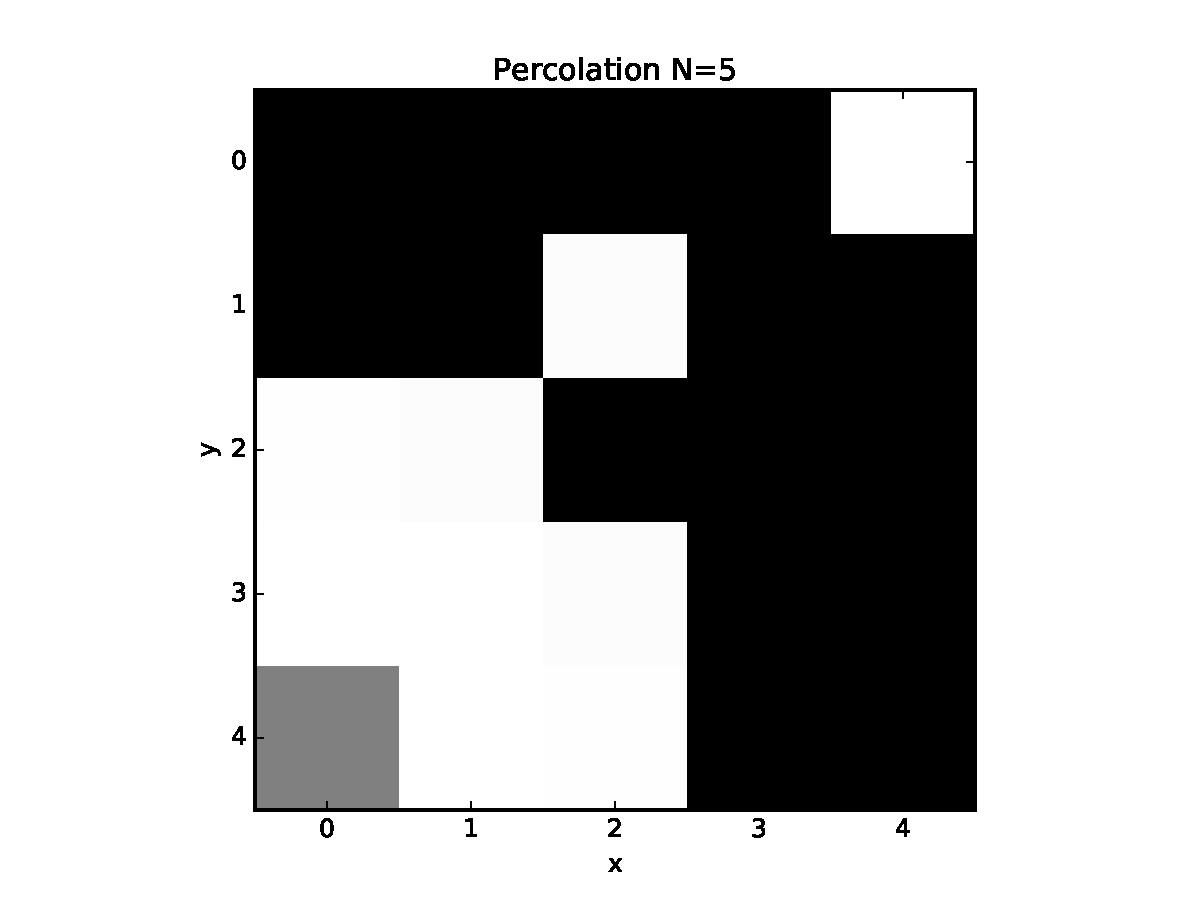
\includegraphics[width=\linewidth]{percolation_5.pdf}
  \label{delta02}
\endminipage\hfill
\minipage{0.5\textwidth}
  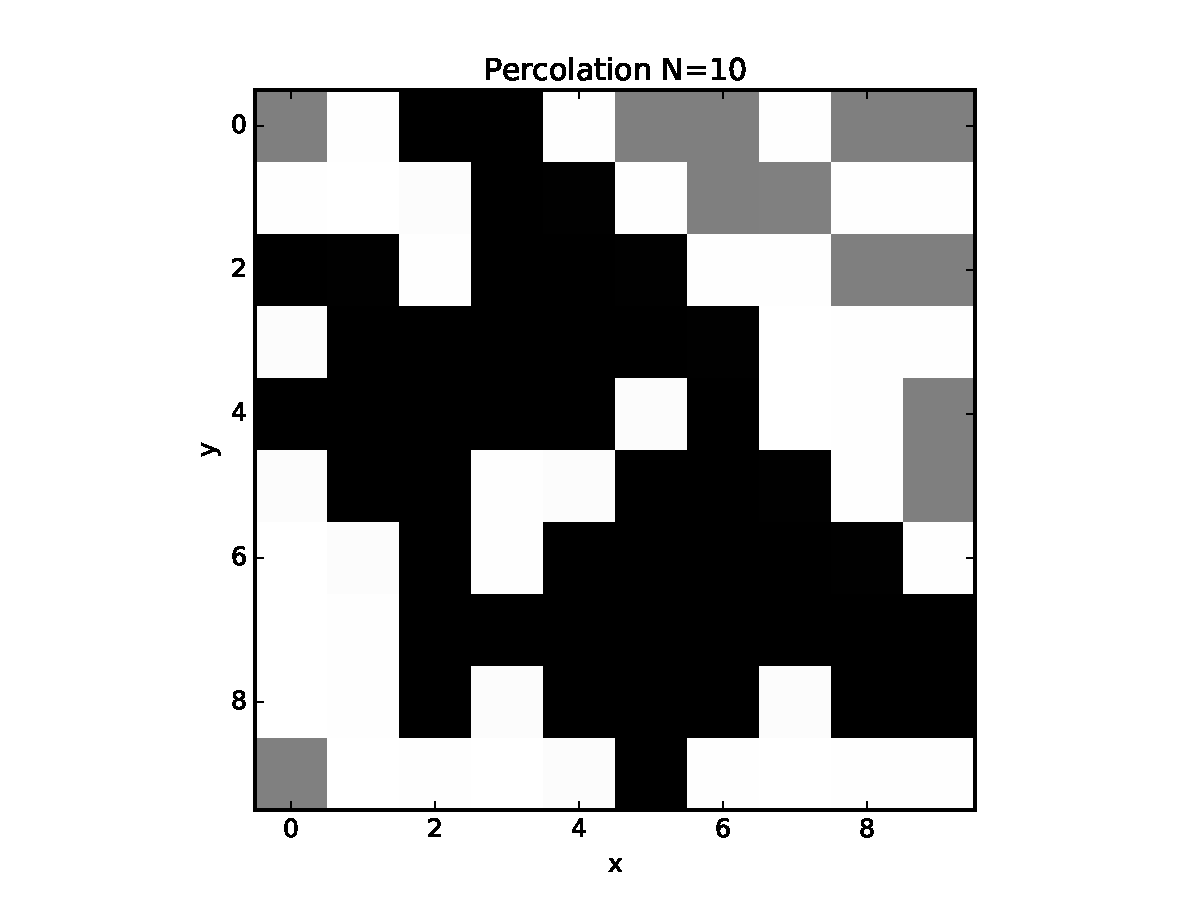
\includegraphics[width=\linewidth]{percolation_10.pdf}
  \label{delta02}
\endminipage\hfill
\minipage{0.5\textwidth}
  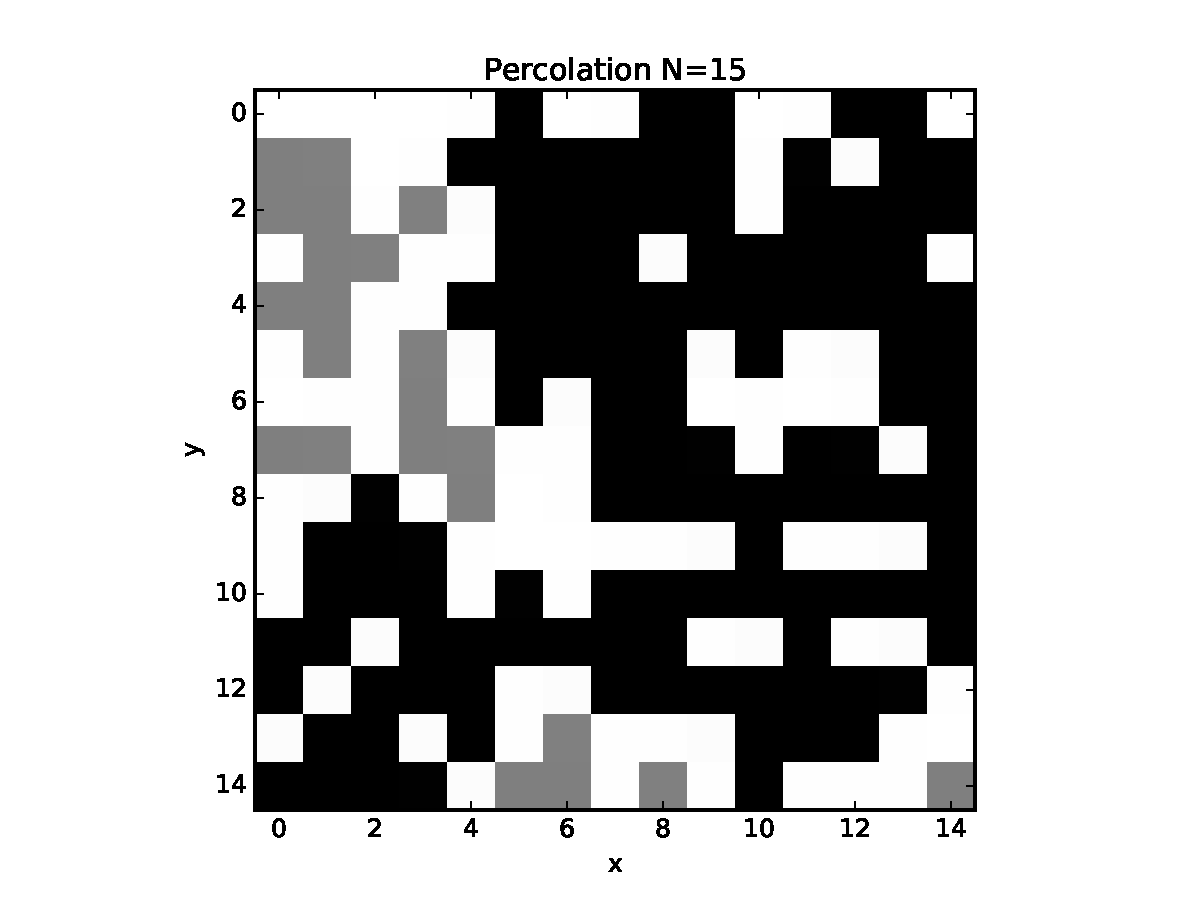
\includegraphics[width=\linewidth]{percolation_15.pdf}
  \label{delta02}
\endminipage\hfill
\minipage{0.5\textwidth}
  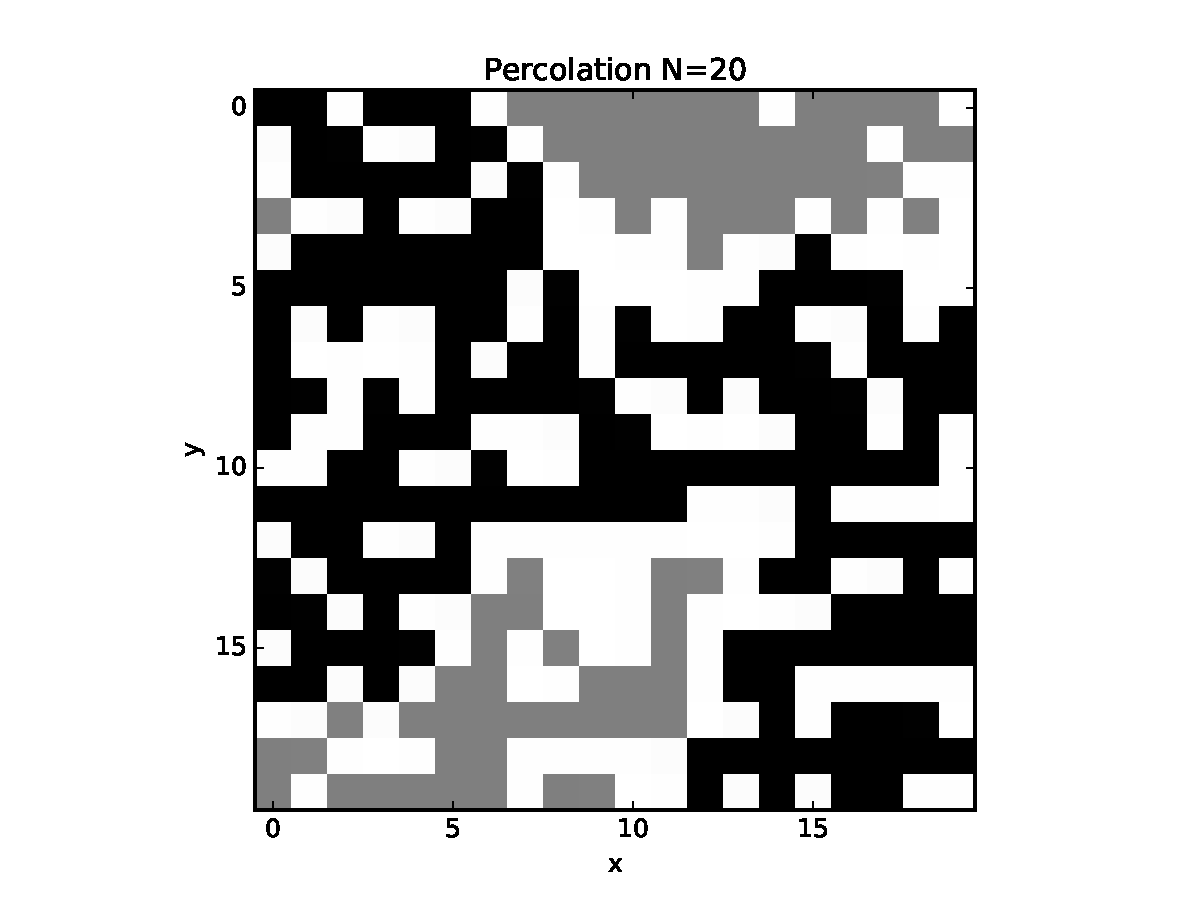
\includegraphics[width=\linewidth]{percolation_20.pdf}
  \label{delta02}
\endminipage\hfill
\end{figure}
\clearpage
\begin{figure}[h]
\minipage{0.5\textwidth}
  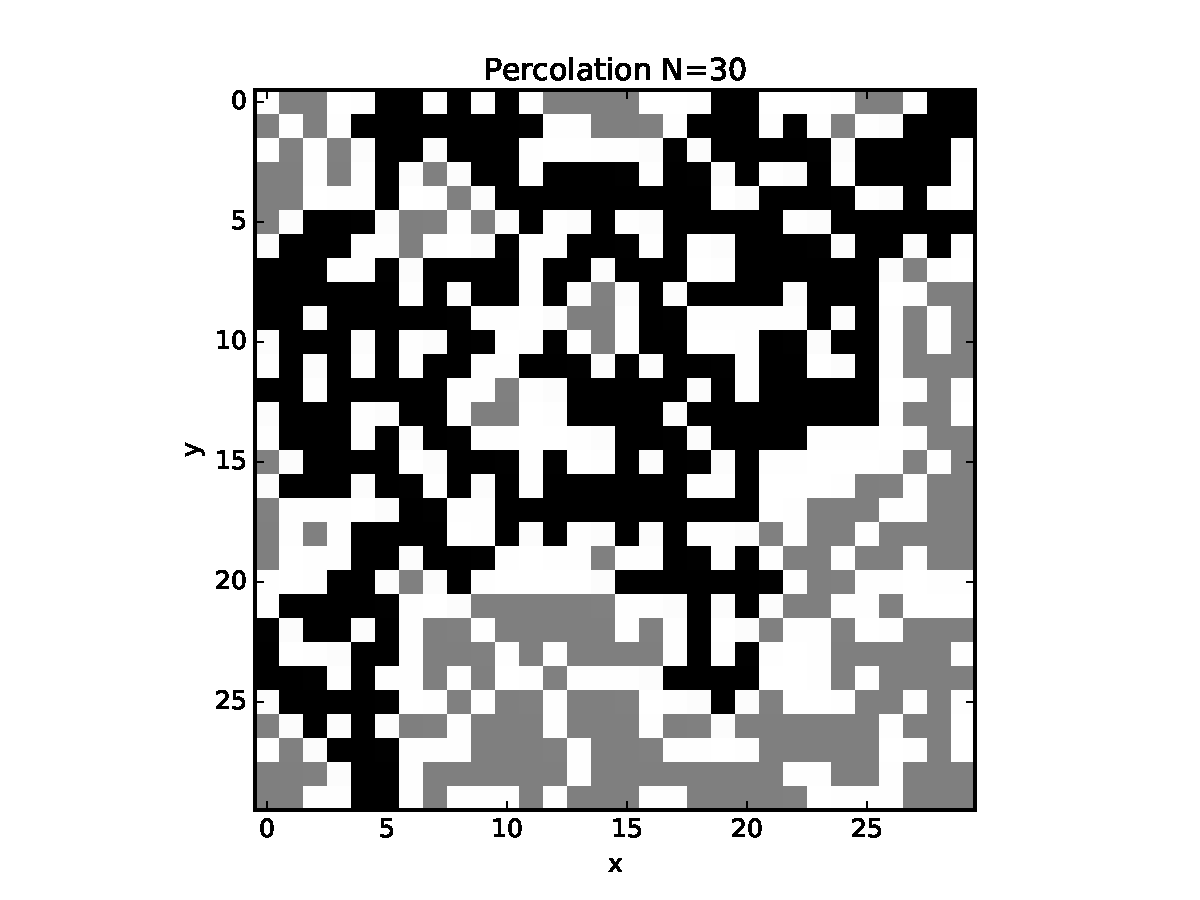
\includegraphics[width=\linewidth]{percolation_30.pdf}
  \label{delta02}
\endminipage\hfill
\minipage{0.5\textwidth}
  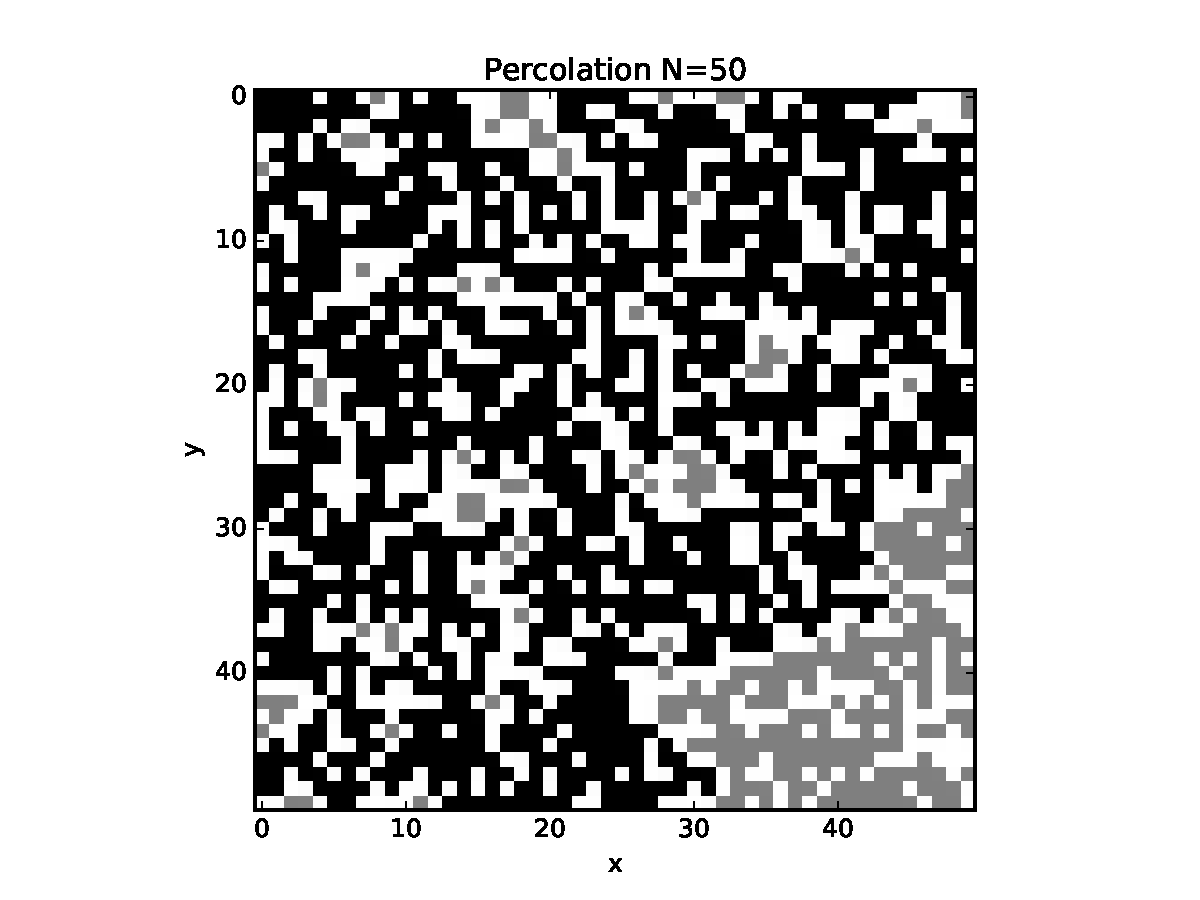
\includegraphics[width=\linewidth]{percolation_50.pdf}
  \label{delta02}
\endminipage\hfill
\minipage{0.5\textwidth}
  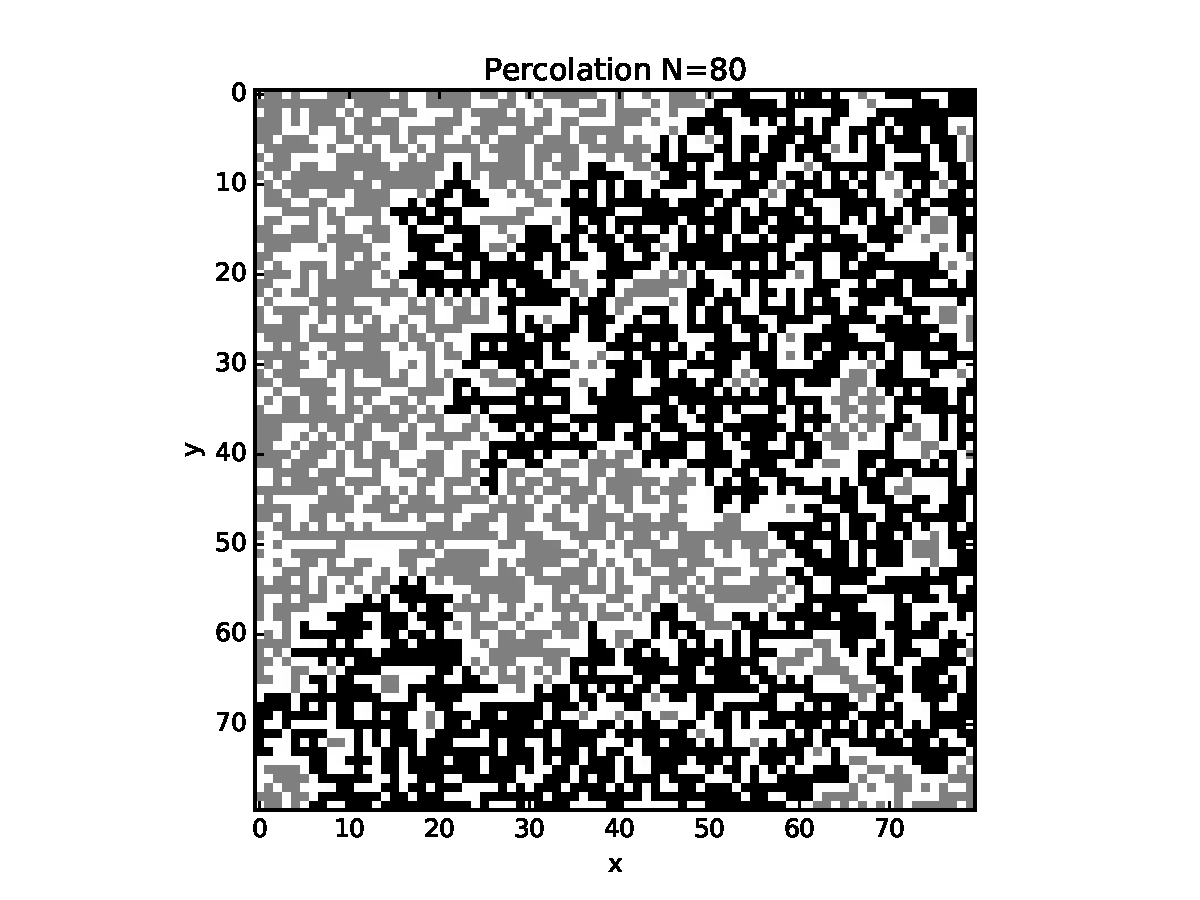
\includegraphics[width=\linewidth]{percolation_80.pdf}
  \label{delta02}
\endminipage\hfill
  \caption{First Appearance of Spanning Clusters for Different Lattices}
\end{figure}
In the pictures above, black sites represent sites of spanning clusters, gray ones represent sites occupied while not belonging to spanning clusters, and white ones represent sites unoccupied.\\
\indent By repeating the procedures over 50 times for each $N$, we can calculate the average $p_c(N^{-1})$. After doing so for all $N\in\{5, 10, 15, 20, 30, 50, 80\}$, we could plot the graph of $p_c(N^{-1})$ as Fig. (\ref{Critical}):
\begin{figure}[H]
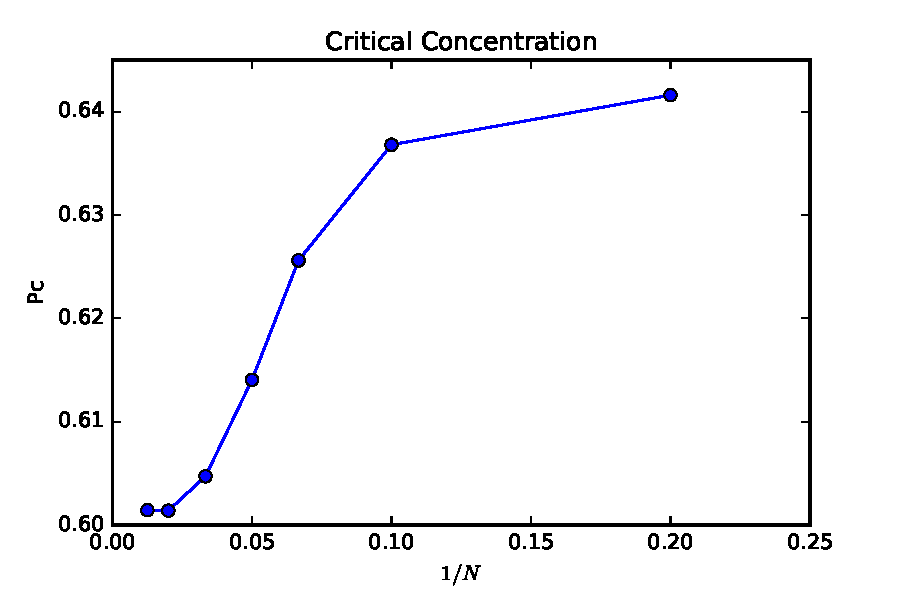
\includegraphics{Critical.pdf}
\caption{Critical Concentration}
\label{Critical}
\end{figure}
According to the graph, we could extrapolate to the infinite size limit $p_c(0)\approx0.602$.
\section{Spanning Cluster Size for Different Lattice}
We define the fraction F of a as
$$F\left(p>p_c\right)=\frac{no.\,of\,sites\,in\,spanning\,cluster}{no.\,of\,occupied\,sites}$$
The procedure of finding the fraction for a certain p is similar to the procedure of finding the critical probability $p_c$. However, the condition to break the loop is not the appearance of the spanning cluster, but the number of occupied sites over the number of all the sites is p. When the spanning cluster first appears, we store the cluster number of the spanning cluster. After the iteration, calculate the number of spanning cluster. The occupied number is calculated by $p\times N\times N$. \\
The whole procedure is repeated for 50 times and then calculate average fraction F. In a lattice with fixed size $(100\times100)$, we plot the fraction F for different probability p in Fig. (\ref{Fraction}). The power law ansatz is 
$$F=F_0\left(p-p_c\right)^\beta$$
By plotting the logarithm for each side and extracting the slope of a straight-line fit, the index $\beta$ can be calculated as in Fig. (\ref{Fraction}). The calculated $\beta$ is 0.1305, which is close to the theoretical value $\frac{5}{36}$. 
\begin{figure}[H]
\centering
  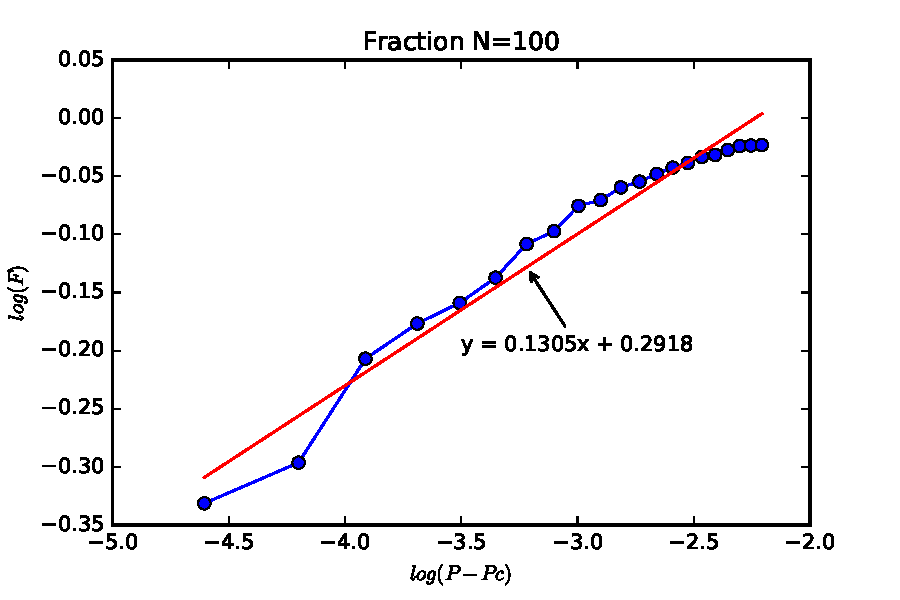
\includegraphics[width=0.8\textwidth]{fraction_all.pdf}
  \label{Fraction}
  \caption{Fraction Plot and Linear Fitting}
\end{figure}
\end{document}
